\subsection{Apollo Server and Client}

GraphQL has a specification and is a query language. The development of a GraphQL server and client is up to the application developer. Facebook's has created their own GraphQL implementation of the specification in JavaScript with GraphQL.js for the backend and Relay for the frontend. Relay is very a prominent example of a GraphQL client, but it only exists for Facebook's React framework. When evaluating different GraphQL clients, Apollo was chosen as it has support for almost every possible programming language and framework.

Apollo Server is an open-source implementation of the GraphQL specification. It offer any feature that a GraphQL server has. And it offers \textbf{Apollo Sandbox} out of the box. \cite{misc:-:apollo-server-introduction} \textbf{Apollo Sandbox} helps local development. The \textbf{Apollo Sandbox} loads the GraphQL Schema from the server with the help of the Introspection Query. \cite{misc:-:apollo-sandbox} Such an environment enables executing queries, mutations directly inside the browser. 

Apollo Client is a community driven project and has npm packages for almost all frontend development environments like the big frameworks as Angular, React and Vue.js. The library fetches, caches and manages the data of the application. The package for Angular is designed with Angular patterns in mind to integrate perfectly with the framework. Apollo Client offer the possibility to cache already made requests. \cite{misc:-:apollo-angular-client-overview} \cite{misc:-:apollo-client-overview} This leads to the next section, where the cache is explained in more detail.

\subsubsection{How does the in-memory cache work?}

This section describes how the cache in apollo-client works. By default all GraphQL requests made with \textbf{ApolloClient} are cached inside the browsers memory. This enables Apollo Client to respond almost immediately to queries for already-cached data, without even sending a network request. This is needed, to ensure to reduce round-trips to the server in subsequent requests of the same query, because the requested data can be served from the cache. The caching mechanism reduces the load of the server, but introduces issues with cache management. \textbf{ApolloClient} includes a caching mechanism called ApolloCache and the proprietary implementation called \textbf{InMemoryCache}. There are several Open-Source alternatives, that implement the \textbf{ApolloCache} interface.

\ifshowImages
\begin{figure}[H]
\centering
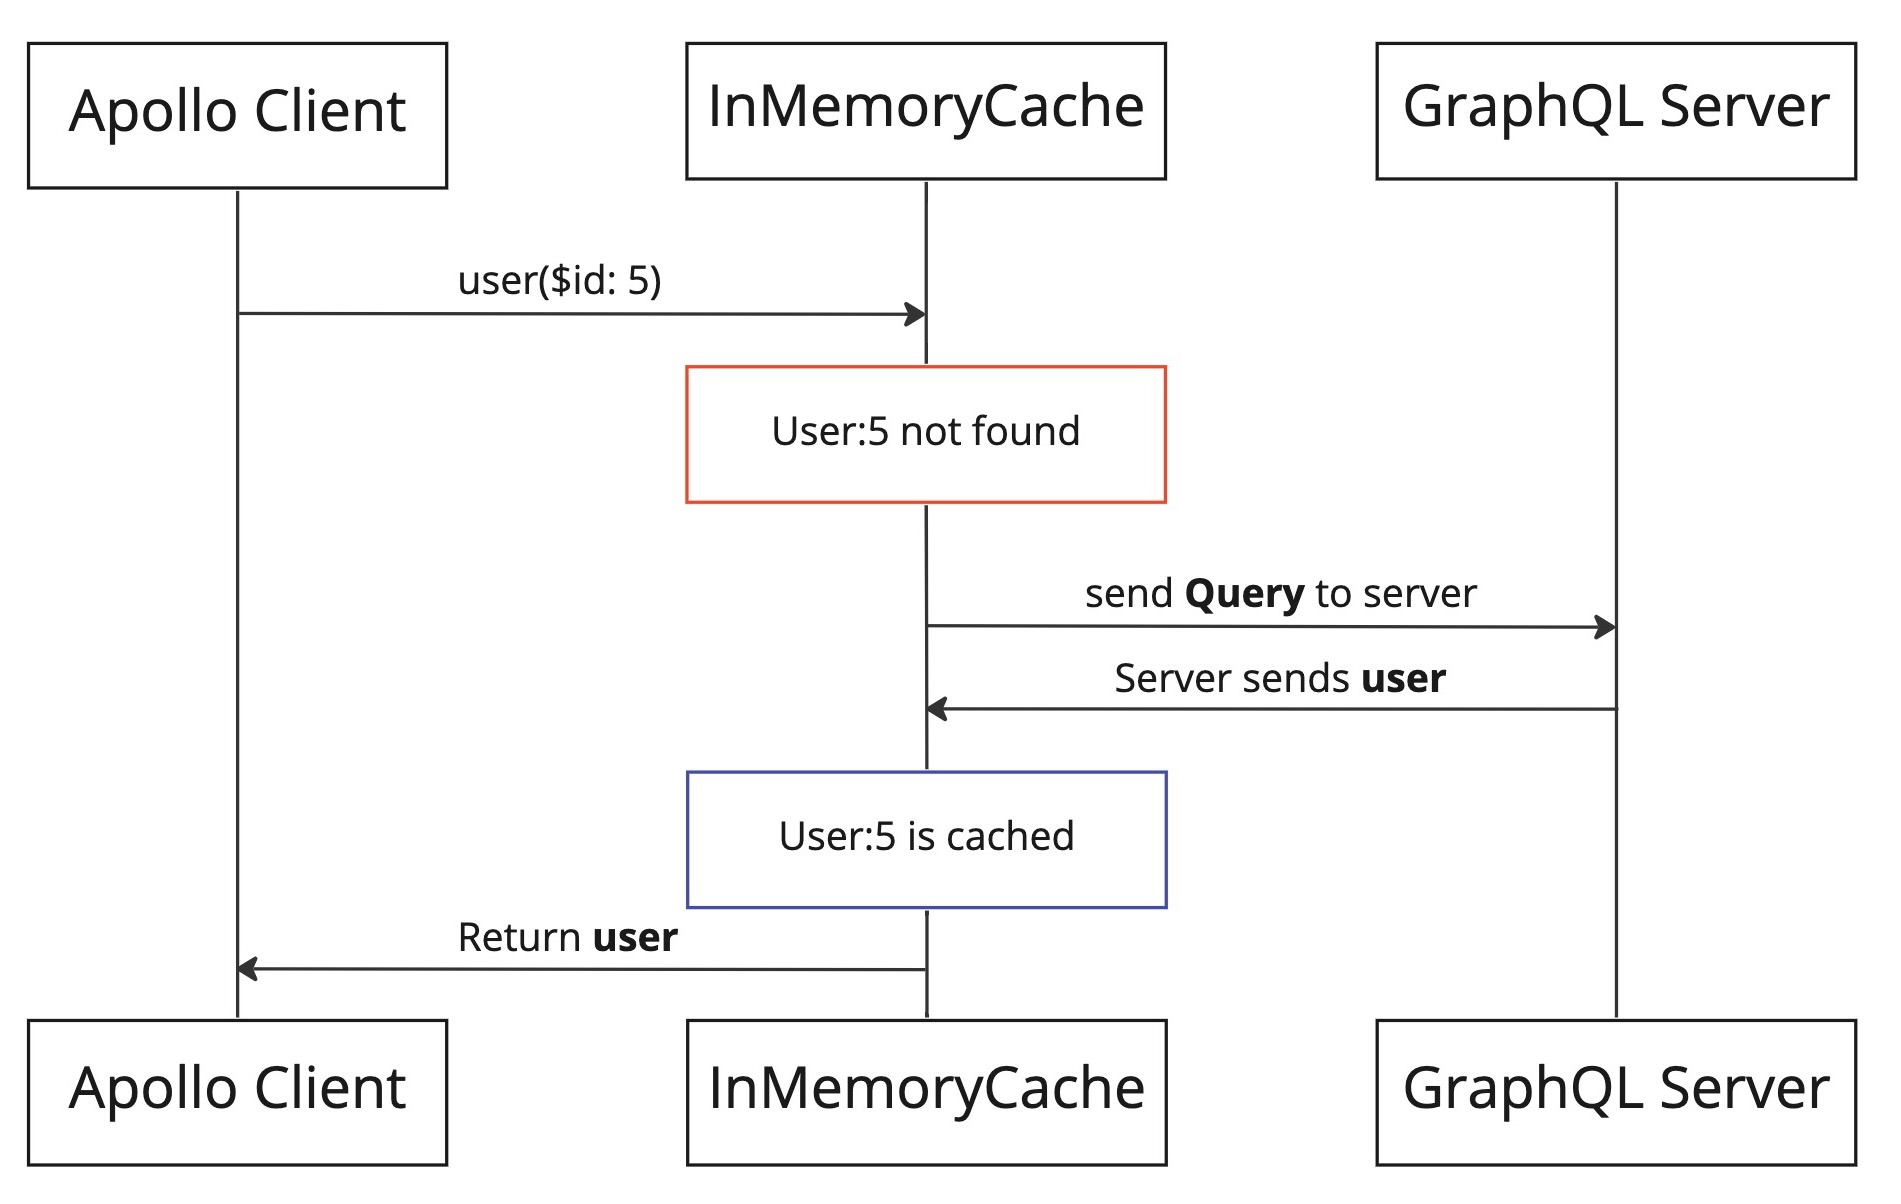
\includegraphics[width=0.6\linewidth]{images/background/apollo/apollo-client-basic-cache.jpeg}
\caption{All requests made during the measurement of the first approach}\label{figure:background:user-query-first-time}
\end{figure}
\fi

The flow of the cache, when the query \textbf{user} is executed the first time is shown in figure \ref{figure:background:user-query-first-time}.

\ifshowImages
\begin{figure}[H]
\centering
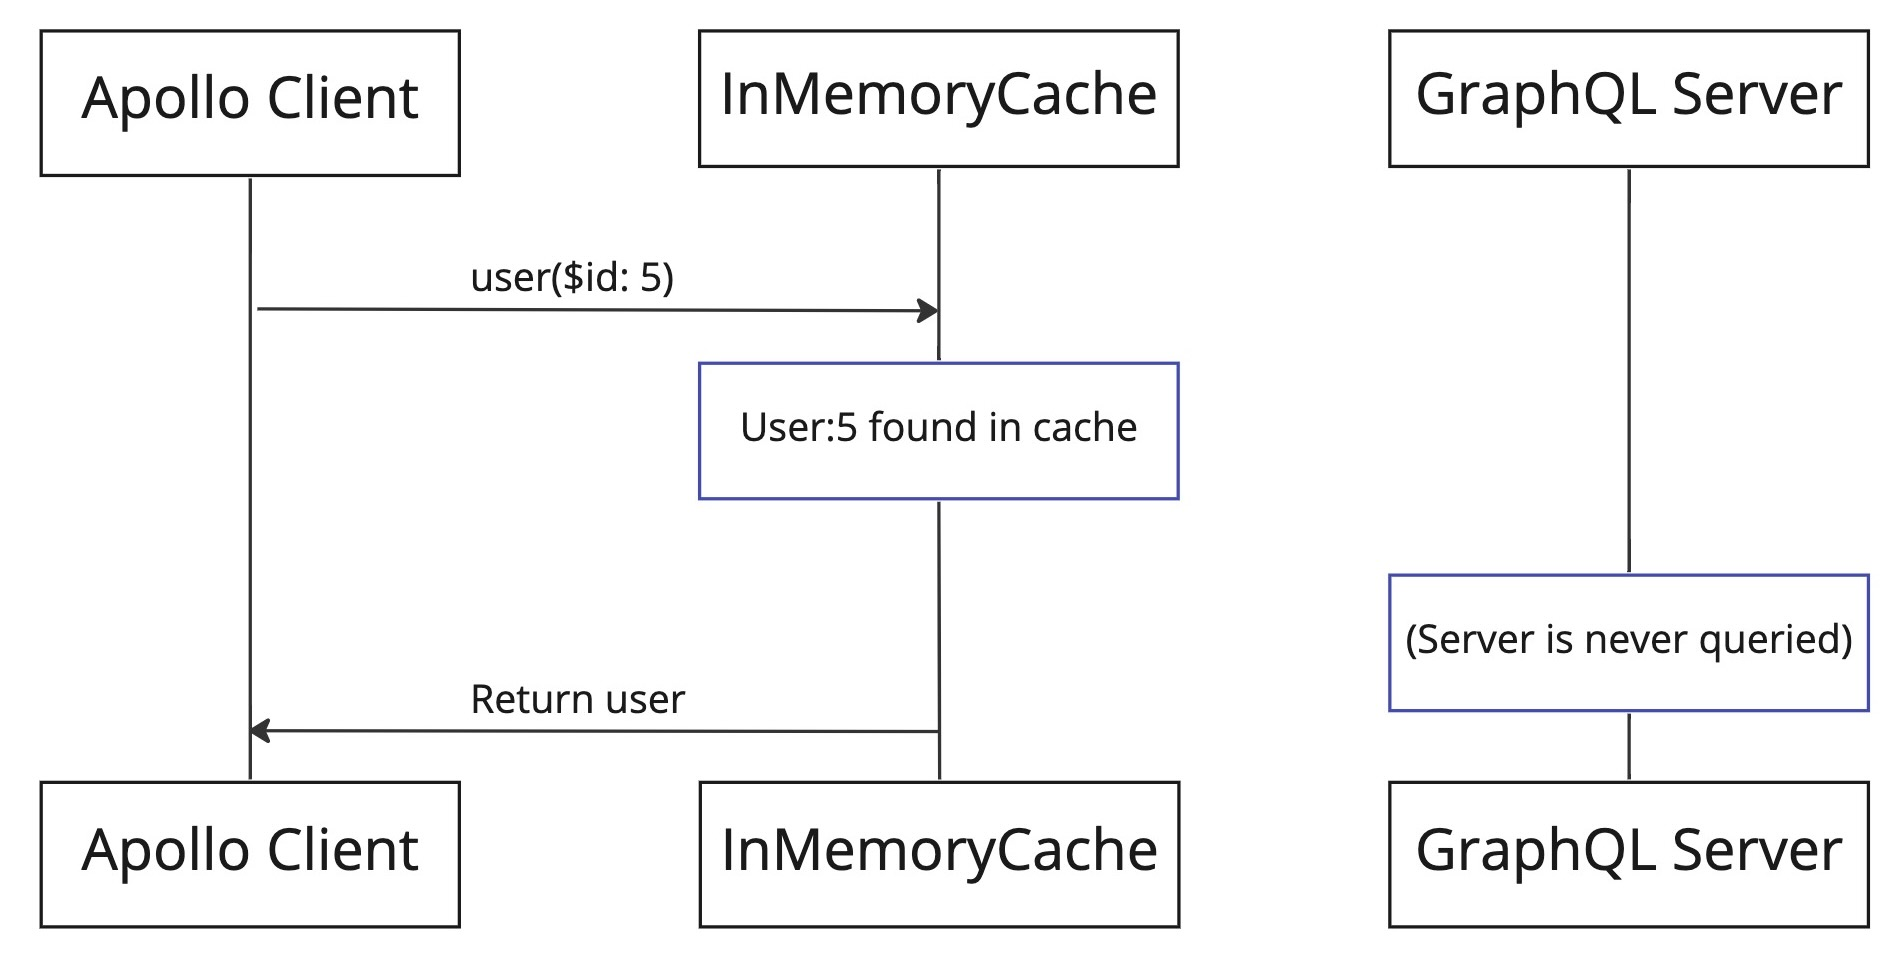
\includegraphics[width=0.6\linewidth]{images/background/apollo/apollo-client-basic-cache-warm.jpeg}
\caption{All requests made during the measurement of the first approach}\label{figure:background:user-query-second-time}
\end{figure}
\fi

When the query is executed later with the same parameters, the flow looks like in figure \ref{figure:background:user-query-second-time}.

In order to correctly understand cache updates, it is important to understand the structure of the cache. The structure of the \textbf{InMemoryCache} is a simple normalized object. When the cache is empty, it is just an empty object. When the following query is requested from the server and the response is stored in the cache, the cache will look like this:

\ifshowListings
\begin{listing}[H]
\begin{minted}{typescript}
query {
  users {
    id
    username
    email
  }
}
\end{minted}
\caption{An example of a query}\label{code:background:query-user-cache}
\end{listing}
\fi

And the server responds with the following result. The \textbf{\_\_typename} property is automatically appended to the query by the \textbf{ApolloClient}.

\ifshowListings
\begin{listing}[H]
\begin{minted}{typescript}
{
  users: [
    {
      __typename: 'User',
      id: '36bad921-8fcf-4f33-9f29-0d3cd70205c8',
      username: 'Florian',
      email: 'florian@test.io'
    }, 
    {
      __typename: 'User',
      id: 'a2096556-9a4e-4994-9de8-86c9e85ed6a1',
      username: 'Daniel',
      email: 'daniel@test.io'
    }
  ]
}
\end{minted}
\caption{The result of the GraphQL query from listing \ref{code:background:query-user-cache}}\label{code:background:query-user-response-result}
\end{listing}
\fi

The \textbf{ApolloClient} will update the cache so that it looks like this.

\ifshowListings
\begin{listing}[H]
\begin{minted}{typescript}
{
  ROOT_QUERY: {
    __typename: 'Query',
    users: [
      { __ref: 'User:36bad921-8fcf-4f33-9f29-0d3cd70205c8', },
      { __ref: 'User:a2096556-9a4e-4994-9de8-86c9e85ed6a1', },
    ],
  },
  'User:36bad921-8fcf-4f33-9f29-0d3cd70205c8': {
    __typeName: 'User',
    id: '36bad921-8fcf-4f33-9f29-0d3cd70205c8',
    username: 'Florian',
    email: 'florian@test.io',
  },
  'User:a2096556-9a4e-4994-9de8-86c9e85ed6a1': {
    __typeName: 'User',
    id: 'a2096556-9a4e-4994-9de8-86c9e85ed6a1',
    username: 'Daniel',
    email: 'daniel@test.io',
  }
}
\end{minted}
\caption{The data inside the cache with the response from listing \ref{code:background:query-user-response-result}}\label{code:background:query-user-cache-representation}
\end{listing}
\fi

Let's describe how the response from the server is transformed into the representation from the cache seen in listing \ref{code:background:query-user-cache-representation}. The cache object contains a key \textbf{ROOT\_QUERY}. This element contains the name of the queries that were executed and the results from all queries. The query \textbf{allUsers} was fetched, therefore the \textbf{ROOT\_QUERY} contains a field with the name \textbf{users}. The listing \ref{code:background:query-user-cache-representation} shows that the content of the \textbf{ApolloClient} is clearly different from the servers response. Instead of the user-information every array item consists of an object with a \textbf{\_\_ref} key. The value of the key is simply the \textbf{\_\_typename} and \textbf{id} of the user concatenated. The data from the response has been normalized and added to the cache object. Next to the \textbf{ROOT\_QUERY} element, the actual user-information is stored. Each has the same key as the \textbf{\_\_ref} from the \textbf{ROOT\_QUERY}. 

The same principle applies to arbitrary deep queries. The following query produces:

\ifshowListings
\begin{listing}[H]
\begin{minted}{typescript}
query {
  allUsers {
    id
    username
    Title {
      id
      name
    }
  }
}
\end{minted}
\caption{An example of a query}\label{code:background:nested-query-user-cache}
\end{listing}
\fi

And the server responds with the following result. The \textbf{\_\_typename} property is automatically appended to the query by the \textbf{ApolloClient}.

\ifshowListings
\begin{listing}[H]
\begin{minted}{typescript}
{
  users: [
    {
      __typename: 'User',
      id: '36bad921-8fcf-4f33-9f29-0d3cd70205c8',
      username: 'Florian',
      title: {
        __typename: 'Title',
        id: '2adb1120-d911-4196-ab1b-d5043cc7a00a',
        name: 'BSc.'
      }
    }, 
    {
      __typename: 'User',
      id: 'a2096556-9a4e-4994-9de8-86c9e85ed6a1',
      username: 'Daniel',
      title: {
        __typename: 'Title',
        id: '2adb1120-d911-4196-ab1b-d5043cc7a00a',
        name: 'BSc.'
      }
    }
  ]
}
\end{minted}
\caption{The result of the GraphQL query from listing \ref{code:background:nested-query-user-cache}}\label{code:background:nested-query-user-response-result}
\end{listing}
\fi

\ifshowListings
\begin{listing}[H]
\begin{minted}{typescript}
{
  ROOT_QUERY: {
    __typename: 'Query',
    users: [
      { __ref: 'User:36bad921-8fcf-4f33-9f29-0d3cd70205c8', },
      { __ref: 'User:a2096556-9a4e-4994-9de8-86c9e85ed6a1', },
    ],
  },
  'User:36bad921-8fcf-4f33-9f29-0d3cd70205c8': {
    __typeName: 'User',
    id: '36bad921-8fcf-4f33-9f29-0d3cd70205c8',
    username: 'Florian',
    Title: {
      __ref: 'Title:2adb1120-d911-4196-ab1b-d5043cc7a00a',
    },
  },
  'User:a2096556-9a4e-4994-9de8-86c9e85ed6a1': {
    __typeName: 'User',
    id: 'a2096556-9a4e-4994-9de8-86c9e85ed6a1',
    username: 'Daniel',
    Title: {
      __ref: 'Title:2adb1120-d911-4196-ab1b-d5043cc7a00a',
    },
  }
  'Title:2adb1120-d911-4196-ab1b-d5043cc7a00a': {
    __typeName: 'Address',
    id: '2adb1120-d911-4196-ab1b-d5043cc7a00a',
    name: 'BSc.',
  },
}
\end{minted}
\caption{The data inside the cache with the response from listing \ref{code:background:nested-query-user-response-result}}\label{code:background:nested-query-user-cache-representation}
\end{listing}
\fi

The \textbf{ROOT\_QUERY} is exactly the same as with the query before. Each user contains a reference to a title. Both users have the same title, therefore the server returned duplicate data. But the cache normalisation causes the title to be only present once in the cache.

This behaviour is very helpful, because when a cache item is updated, the entire cache object doesn't have to be traversed in search for the instance that has been changed. Only a single item has to updated.

The cache normalisation works when the query contains either a \textbf{\_id} or \textbf{id} field. Without an id the object can't be normalized. Here is an example:

\ifshowListings
\begin{listing}[H]
\begin{minted}{typescript}
query {
  allUsers {
    id
    username
    Title {
      name
    }
  }
}
\end{minted}
\caption{An example of a query}\label{code:background:no-id-query-user-cache}
\end{listing}
\fi

The response: 

\ifshowListings
\begin{listing}[H]
\begin{minted}{typescript}
{
  users: [
    {
      __typename: 'User',
      id: '36bad921-8fcf-4f33-9f29-0d3cd70205c8',
      username: 'Florian',
      title: {
        __typename: 'Title',
        name: 'BSc.'
      }
    }, 
    {
      __typename: 'User',
      id: 'a2096556-9a4e-4994-9de8-86c9e85ed6a1',
      username: 'Daniel',
      title: {
        __typename: 'Title',
        name: 'BSc.'
      }
    }
  ]
}
\end{minted}
\caption{The result of the GraphQL query from listing \ref{code:background:no-id-query-user-cache}}\label{code:background:no-id-query-user-response-result}
\end{listing}
\fi

And the cache looks like the following:

\ifshowListings
\begin{listing}[H]
\begin{minted}{typescript}
{
  ROOT_QUERY: {
    __typename: 'Query',
    users: [
      { __ref: 'User:36bad921-8fcf-4f33-9f29-0d3cd70205c8', },
      { __ref: 'User:a2096556-9a4e-4994-9de8-86c9e85ed6a1', },
    ],
  },
  'User:36bad921-8fcf-4f33-9f29-0d3cd70205c8': {
    __typeName: 'User',
    id: '36bad921-8fcf-4f33-9f29-0d3cd70205c8',
    username: 'Florian',
    Title: {
      name: 'BSc.',
    },
  },
  'User:a2096556-9a4e-4994-9de8-86c9e85ed6a1': {
    __typeName: 'User',
    id: 'a2096556-9a4e-4994-9de8-86c9e85ed6a1',
    username: 'Daniel',
    Title: {
      name: 'BSc.',
    },
  }
}
\end{minted}
\caption{The data inside the cache with the response from listing \ref{code:background:no-id-query-user-response-result}}\label{code:background:no-id-query-user-cache-representation}
\end{listing}
\fi

This should be avoided. If data of an unnormalized object has to be updated every occurrence of the item in the cache has to be updated manually. You must also never request the same thing sometimes with an id and sometimes without, because \textbf{ApolloClient} will throw an error when trying to update the cache after such a query.

The Apollo Client's cache stores the data a flat lookup table of objects that reference each other. These objects correspond to the objects that are returned by the GraphQL queries. A single cached object might include fields that were fetched by multiple queries. That means that multiple queries can fetch different fields for the same object. Before storing the data, the cache needs to normalize it. \cite{misc:-:apollo-client-cache-overview}

Whenever the Apollo Client receives the response data of a query it does the following. a

\paragraph{1. Identify objects} 

The cache identifies all distinct objects included in query response.

\begin{itemize}
  \item A \textbf{User} with id \textbf{36bad921-8fcf-4f33-9f29-0d3cd70205c8}
  \item A \textbf{User} with id \textbf{a2096556-9a4e-4994-9de8-86c9e85ed6a1}
\end{itemize}

\paragraph{2. Generate cache IDs} 

After identifying all objects, the cache generates a cache ID for each object. A cache ID uniquely identifies a particular object, while it is in the \textbf{InMemoryCache}.

So, the cache IDs for the objects are: 

\begin{itemize}
  \item \textbf{User:36bad921-8fcf-4f33-9f29-0d3cd70205c8}
  \item \textbf{User:a2096556-9a4e-4994-9de8-86c9e85ed6a1}
\end{itemize}

By default, an object's cache ID is the concentation of the object's \textbf{\_\_typename} and \textbf{id} (or \textbf{\_id}) fields.

If the cache can't generate a cache ID for a particular object, that object is directly cached inside its parent object, and must be referenced via the parent. Therefore the cache is not always completely flat.

\paragraph{3. Replace object fields with references} 

Next, the cache takes each field that contains an object and replaces its value with a reference to the appropriate object.

\ifshowListings
\begin{listing}[H]
\begin{minted}{typescript}
{
  __typename: 'User',
  id: '36bad921-8fcf-4f33-9f29-0d3cd70205c8',
  username: 'Florian',
  title: {
    __typename: 'Title',
    id: '2adb1120-d911-4196-ab1b-d5043cc7a00a',
    name: 'BSc.'
  }
}, 
\end{minted}
\caption{The result of the GraphQL query from listing \ref{code:background:no-id-query-user-cache}}
\end{listing}
\fi

And here's that same object after replacement:

\ifshowListings
\begin{listing}[H]
\begin{minted}{typescript}
{
  __typename: 'User',
  id: '36bad921-8fcf-4f33-9f29-0d3cd70205c8',
  username: 'Florian',
  title: {
    __ref: 'Title:36bad921-8fcf-4f33-9f29-0d3cd70205c8',
  }
}, 
\end{minted}
\caption{The result of the GraphQL query from listing \ref{code:background:no-id-query-user-cache}}
\end{listing}
\fi

The \textbf{title} field now contains a reference to the appropriate normalized \textbf{Title} object.

If another \textbf{User} with the same \textbf{title}, that normalized \textbf{Title} object is reused. Normalization can drastically reduce data duplication inside the cache. It also helps to make the data stay synchronous to the server.

\paragraph{4. Store normalized objects} 

The resulting objects are stored inside the cache's flat lookup table. Whenever an incoming object has the same cache ID as an existing cached object, the fields of those objects are merged together. If the incoming and the existing object share existing fields, the incoming object overwrites the cached value for those fields. Fields that exist only one one object are preserved. This normalization constructs a partial copy of the graph on our client. \cite{misc:-:apollo-client-cache-overview}

\subsubsection{Seeing the content of the cache}

Apollo offers development tools for the browser in form of browser extensions. The \textbf{Apollo Client Developer Tools} can be installed for Chrome and Firefox. The extension can be found in the Chrome Web Store and the Firefox Add-ons Store. \cite{misc:-:apollo-developer-tools} To fully understand the structure of the cache, the content can be printed to the browsers development console. The browser extension adds a tab to the browser inspection tools. A part of the developer tools are shown in figure \ref{fig:background:apollo:apollo-dev-tools}.

\ifshowImages
  \begin{figure}[H]
  \centering
  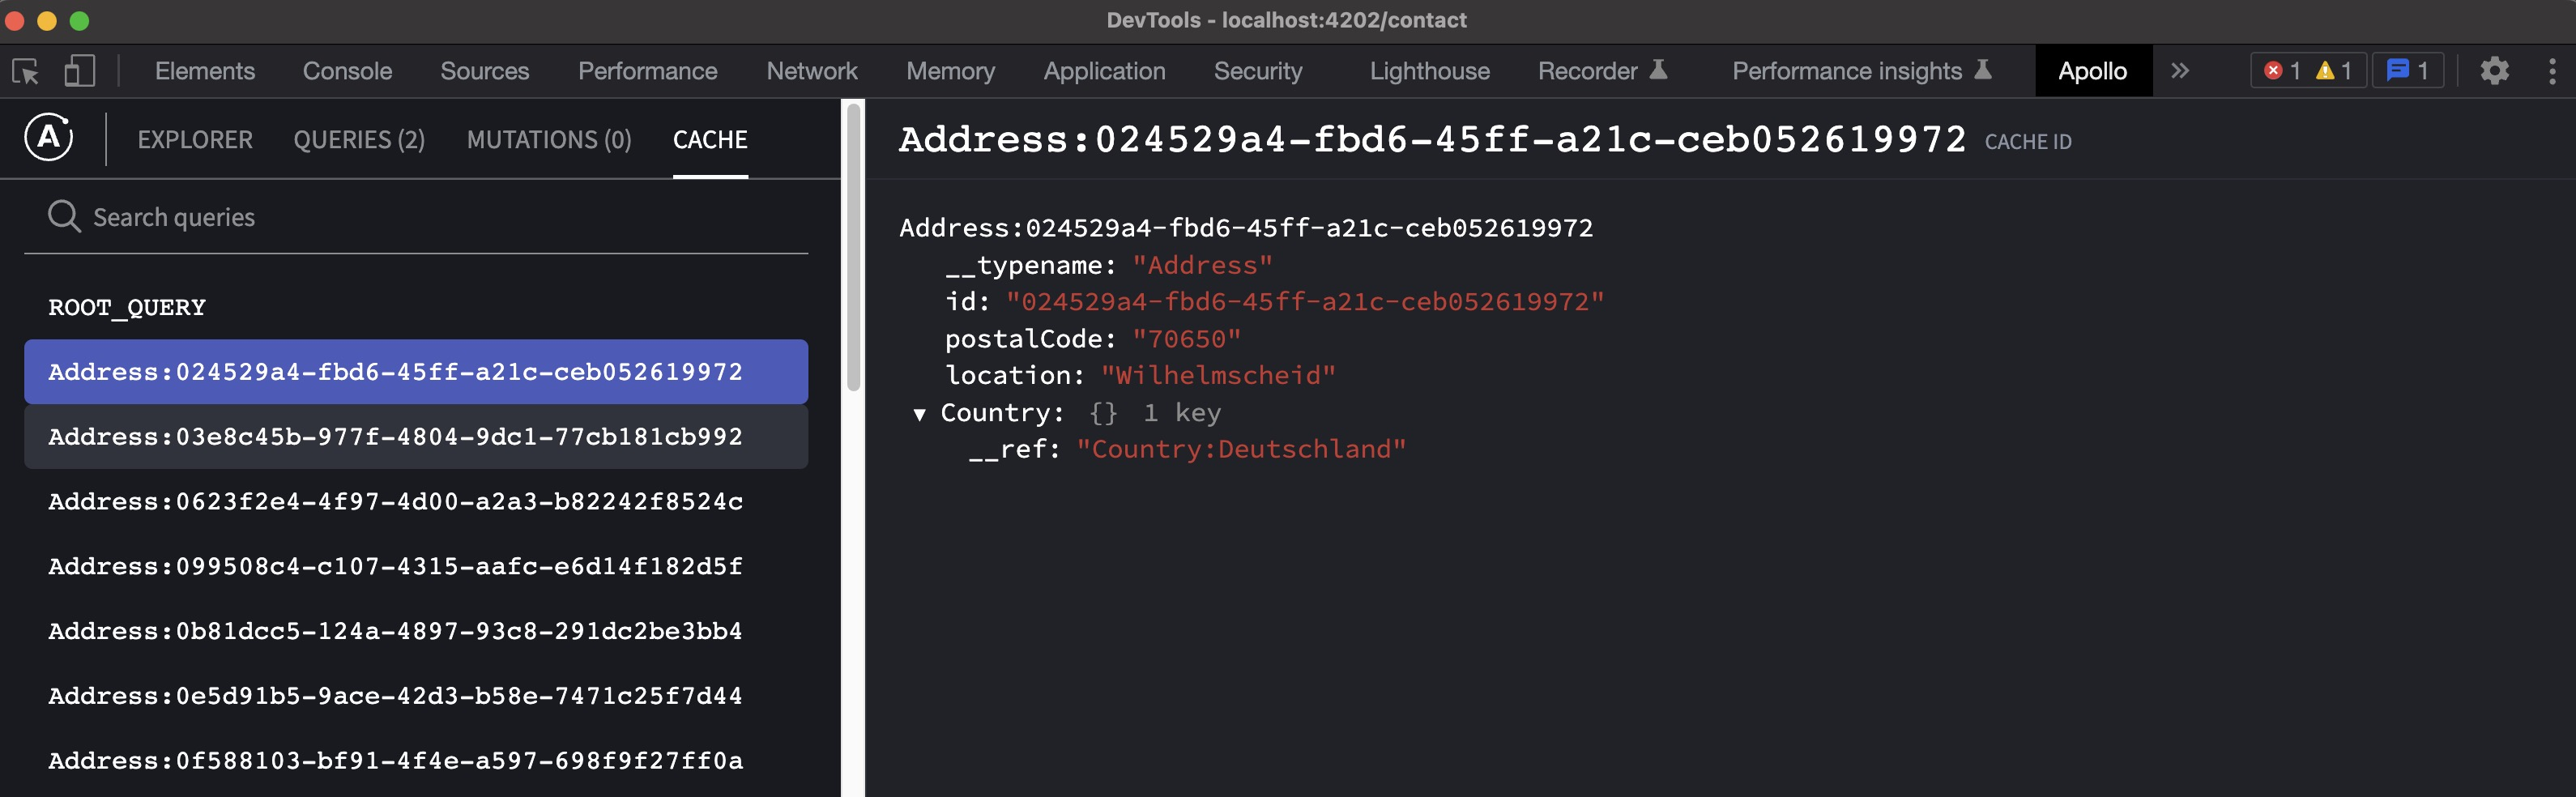
\includegraphics[width=1\linewidth]{images/background/apollo/apollo-dev-tools.jpeg}
  \caption{All requests made during the measurement of the first approach}\label{fig:background:apollo:apollo-dev-tools}
  \end{figure}
\fi

The development tools offer the following four main features:

\begin{itemize}
  \item \textbf{GraphiQL}: Send queries to your server through your web application's configured Apollo Client instance, or query the Apollo Client cache to see what data is loaded.
  \item \textbf{Watched query inspector}: View active queries, variables and cached results, and re-run individual queries.
  \item \textbf{Mutation inspector}: View active mutations and their variables, and re-run individual mutations
  \item \textbf{Cache inspector}: Visualize the Apollo Client and search it by field name and/or value.
\end{itemize}

Another method to access the content of the cache is through the \textbf{window} object in JavaScript. The object can be accessed through \textbf{window.\_\_APOLLO\_CLIENT\_\_.cache.extract(\)\}.

\ifshowImages
  \begin{figure}[H]
  \centering
  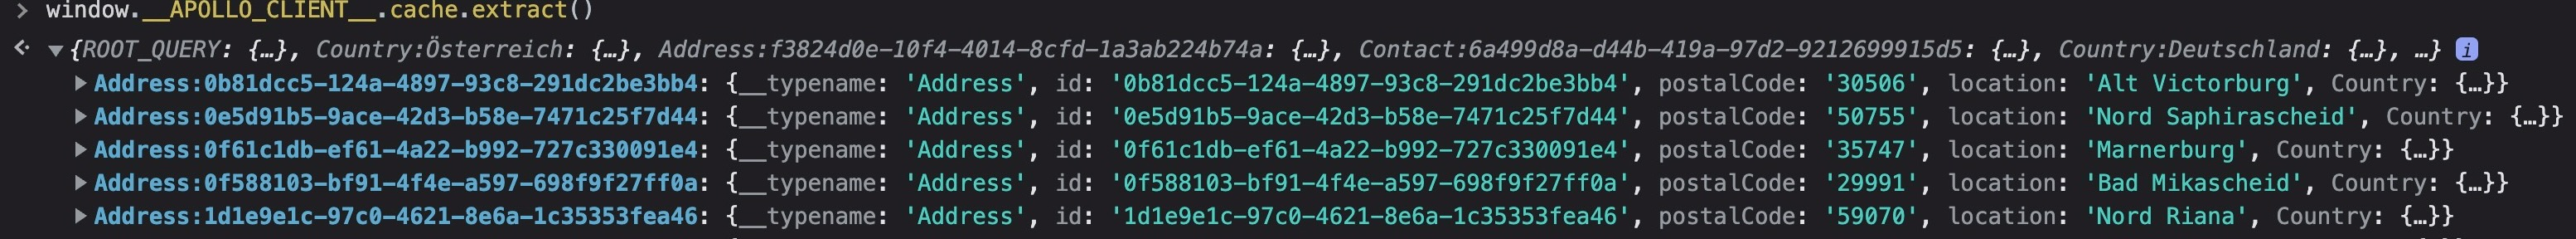
\includegraphics[width=1\linewidth]{images/background/apollo/apollo-cache-browser-window.jpeg}
  \caption{All requests made during the measurement of the first approach}\label{fig:background:apollo:apollo-cache-browser-window}
  \end{figure}
\fi